\documentclass{beamer}
\usepackage[utf8]{inputenc}
\usepackage{graphicx}
\usepackage{tikz}
\usepackage{xcolor}
% TIKZ TEMPLATE STARTED
\usetikzlibrary{shapes.geometric, arrows}
\tikzstyle{startstop} = [rectangle, rounded corners, minimum width=3cm, minimum height=1cm, text centered, draw=black, fill=red!30]
\tikzstyle{gnode} = [circle, minimum width=.35cm, minimum height=.35cm, text centered, draw=black, fill=red!30]
\tikzstyle{gleaf} = [circle, minimum width=1cm, minimum height=1cm, text centered, draw=black, fill=green!30]
\tikzstyle{gleaf2} = [circle, minimum width=1cm, minimum height=1cm, text centered, draw=black, fill=blue!30]
\tikzstyle{io} = [trapezium, trapezium left angle=70, trapezium right angle=110, minimum width=3cm, minimum height=1cm, text centered, draw=black, fill=blue!30]
\tikzstyle{process} = [rectangle, minimum width=3cm, minimum height=1cm, text centered, text width=3cm, draw=black, fill=orange!30]
\tikzstyle{textonly} = [rectangle, minimum width=1cm, minimum height=1cm, text center, text width=1cm, draw=white, fill=white]
\tikzstyle{decision} = [diamond, minimum width=3cm, minimum height=1cm, text centered, draw=black, fill=green!30]
\tikzstyle{arrow} = [thick,->,>=stealth]
\tikzstyle{place}=[circle,draw=blue!50,fill=blue!20,thick]
\tikzstyle{visited} = [circle, draw, red!50, fill=green!20,thick]
\tikzstyle{current} = [circle, draw, red!50, fill=blue!20,thick]
% TIKS TEMPLATE ENDED
% \usetheme{Madrid}

\title{Class 3 - Beamer}
\subtitle{Fibonacci Heap}
\author[N. N]{No Name}
\institute[CSE, BUET]{
    Department of Computer Science and Engineering\\
    Bangladesh University of Engineering and Technology
}
% \logo{\includegraphics[height=1cm]{}}
\date{\today}

\begin{document}
\begin{frame}{}
\maketitle
\end{frame}
% \begin{frame}{Table of Contents}
% \tableofcontents
% \end{frame}
\begin{frame}{Fibonacci Heap: Extract Min}
\begin{tikzpicture}[scale=0.8, every node/.style={scale=0.8}]
\begin{itemize}
    \item \node at (3,0) [gnode](7) {7};
    \item \node at (6,0) [gnode](24) {24};
    \item \node at (9,0) [gnode](23) {23};
    \item \node at (12,0) [gnode](17) {17};
    \item<1> \node at (15,0) [gnode](3) {3};
    
    \item \node at (3, -2) [gnode](30){30};
    \item \node at (4.5, -2) [gnode](26){26};
    \item \node at (6, -2) [gnode](46){46};
    \item \node at (13.5, -2) [gnode](18){18};
    \item \node at (15, -2) [gnode](52){52};
    \item \node at (16.5, -2) [gnode](41){41};
    
    \item \node at (4.5, -4) [gnode](35){35};
    \item \node at (13.5, -4) [gnode](39){39};
    \item \node at (16.5, -4) [gnode](44){44};
    
    \item<1> \node at (15, 2) [textonly](min2){min};
    
    \item \draw \arrow (7) -- (30);
    \item \draw \arrow (35) -- (26) -- (24) -- (46);
    \item \draw \arrow (39) -- (18);
    \item<1> \draw \arrow (18) -- (3);
    \item<1> \draw \arrow (3) -- (41);
    \item \draw \arrow (41) -- (44);
    \item<1> \draw \arrow (3) -- (52);
    
    \item \draw \arrow[dashed] (7) -- (24) -- (23) -- (17);
    \item<1> \draw \arrow[dashed] (17) -- (3);
    \item<1> \draw \arrow[->] (min2) -- (3);
    \pause
    \item \node at (3, 2) [textonly](min1){min};
    \item \draw \arrow[->] (min1) -- (7);
\end{itemize}
\end{tikzpicture}
\end{frame}


\begin{frame}{Fibonacci Heap: Extract Min}
\begin{tikzpicture}[scale=0.8, every node/.style={scale=0.8}]
\begin{itemize}
    \item \node at (3,0) [gnode](7) {7};
    \item \node at (6,0) [gnode](24) {24};
    \item \node at (9,0) [gnode](23) {23};
    \item \node at (12,0) [gnode](17) {17};
    
    \item \node at (3, -2) [gnode](30){30};
    \item \node at (4.5, -2) [gnode](26){26};
    \item \node at (6, -2) [gnode](46){46};
    \item \node at (13.5, 0) [gnode](18){18};
    \item \node at (15, 0) [gnode](52){52};
    \item \node at (16.5, 0) [gnode](41){41};
    
    \item \node at (4.5, -4) [gnode](35){35};
    \item \node at (13.5, -2) [gnode](39){39};
    \item \node at (16.5, -2) [gnode](44){44};
    
    \item \draw \arrow (7) -- (30);
    \item \draw \arrow (35) -- (26) -- (24) -- (46);
    \item \draw \arrow (39) -- (18);
    \item \draw \arrow (41) -- (44););
    
    \item \draw \arrow[dashed] (7) -- (24) -- (23) -- (17) -- (18) -- (52) -- (41);
    \item \node at (3, 2) [textonly](min1){min};
    \item \draw \arrow[->] (min1) -- (7);
\end{itemize}
\end{tikzpicture}
\end{frame}

\begin{frame}{Fibonacci: Text And Image}

\begin{columns}
    \column{.5\textwidth}
    \begin{itemize}
        \item Extract/Delete Min
        \setbeamercovered{transparent}
        \begin{itemize}
            \item \alert{Delete} min and \alert{add} its children into the root list
            \item {\color{gray}Consolidate trees so that no two roots have same degree}
        \end{itemize}
    \end{itemize}
    \pause
    \column{.4\textwidth}
    \begin{figure}[h]
        \centering
        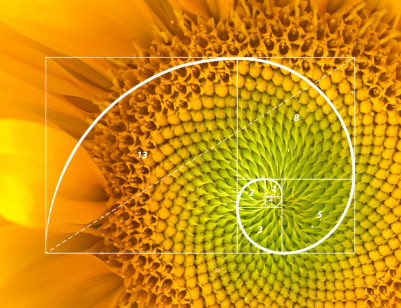
\includegraphics[width=3cm]{image.png}
        % \caption{Caption}
        \label{fig:my_label}
    \end{figure}
    
\end{columns}
    
\end{frame}


\end{document}
